% Created by tikzDevice version 0.10.1 on 2017-09-05 19:12:51
% !TEX encoding = UTF-8 Unicode
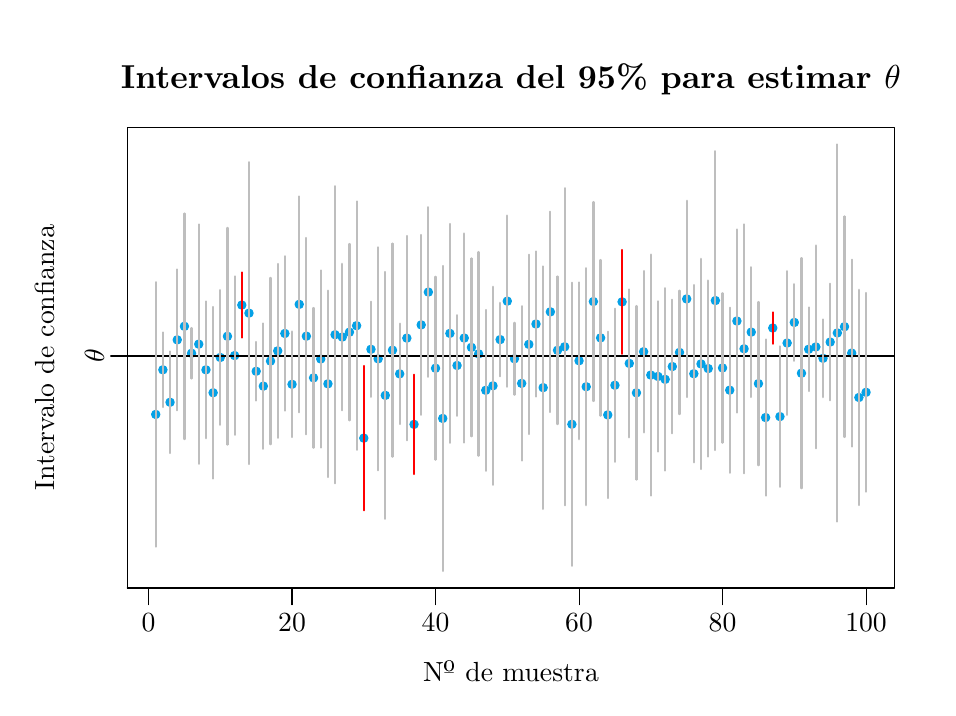
\begin{tikzpicture}[x=1pt,y=1pt]
\definecolor{fillColor}{RGB}{255,255,255}
\path[use as bounding box,fill=fillColor,fill opacity=0.00] (0,0) rectangle (325.21,238.49);
\begin{scope}
\path[clip] ( 36.00, 36.00) rectangle (313.21,202.49);
\definecolor{drawColor}{RGB}{5,161,230}
\definecolor{fillColor}{RGB}{5,161,230}

\path[draw=drawColor,line width= 0.4pt,line join=round,line cap=round,fill=fillColor] ( 46.27, 98.74) circle (  1.50);

\path[draw=drawColor,line width= 0.4pt,line join=round,line cap=round,fill=fillColor] ( 48.86,114.86) circle (  1.50);

\path[draw=drawColor,line width= 0.4pt,line join=round,line cap=round,fill=fillColor] ( 51.45,103.13) circle (  1.50);

\path[draw=drawColor,line width= 0.4pt,line join=round,line cap=round,fill=fillColor] ( 54.05,125.68) circle (  1.50);

\path[draw=drawColor,line width= 0.4pt,line join=round,line cap=round,fill=fillColor] ( 56.64,130.58) circle (  1.50);

\path[draw=drawColor,line width= 0.4pt,line join=round,line cap=round,fill=fillColor] ( 59.23,120.83) circle (  1.50);

\path[draw=drawColor,line width= 0.4pt,line join=round,line cap=round,fill=fillColor] ( 61.82,124.13) circle (  1.50);

\path[draw=drawColor,line width= 0.4pt,line join=round,line cap=round,fill=fillColor] ( 64.42,114.85) circle (  1.50);

\path[draw=drawColor,line width= 0.4pt,line join=round,line cap=round,fill=fillColor] ( 67.01,106.57) circle (  1.50);

\path[draw=drawColor,line width= 0.4pt,line join=round,line cap=round,fill=fillColor] ( 69.60,119.31) circle (  1.50);

\path[draw=drawColor,line width= 0.4pt,line join=round,line cap=round,fill=fillColor] ( 72.19,126.97) circle (  1.50);

\path[draw=drawColor,line width= 0.4pt,line join=round,line cap=round,fill=fillColor] ( 74.79,120.00) circle (  1.50);

\path[draw=drawColor,line width= 0.4pt,line join=round,line cap=round,fill=fillColor] ( 77.38,138.26) circle (  1.50);

\path[draw=drawColor,line width= 0.4pt,line join=round,line cap=round,fill=fillColor] ( 79.97,135.34) circle (  1.50);

\path[draw=drawColor,line width= 0.4pt,line join=round,line cap=round,fill=fillColor] ( 82.57,114.33) circle (  1.50);

\path[draw=drawColor,line width= 0.4pt,line join=round,line cap=round,fill=fillColor] ( 85.16,108.96) circle (  1.50);

\path[draw=drawColor,line width= 0.4pt,line join=round,line cap=round,fill=fillColor] ( 87.75,118.01) circle (  1.50);

\path[draw=drawColor,line width= 0.4pt,line join=round,line cap=round,fill=fillColor] ( 90.34,121.70) circle (  1.50);

\path[draw=drawColor,line width= 0.4pt,line join=round,line cap=round,fill=fillColor] ( 92.94,127.99) circle (  1.50);

\path[draw=drawColor,line width= 0.4pt,line join=round,line cap=round,fill=fillColor] ( 95.53,109.62) circle (  1.50);

\path[draw=drawColor,line width= 0.4pt,line join=round,line cap=round,fill=fillColor] ( 98.12,138.51) circle (  1.50);

\path[draw=drawColor,line width= 0.4pt,line join=round,line cap=round,fill=fillColor] (100.71,127.01) circle (  1.50);

\path[draw=drawColor,line width= 0.4pt,line join=round,line cap=round,fill=fillColor] (103.31,111.95) circle (  1.50);

\path[draw=drawColor,line width= 0.4pt,line join=round,line cap=round,fill=fillColor] (105.90,118.77) circle (  1.50);

\path[draw=drawColor,line width= 0.4pt,line join=round,line cap=round,fill=fillColor] (108.49,109.79) circle (  1.50);

\path[draw=drawColor,line width= 0.4pt,line join=round,line cap=round,fill=fillColor] (111.09,127.54) circle (  1.50);

\path[draw=drawColor,line width= 0.4pt,line join=round,line cap=round,fill=fillColor] (113.68,126.70) circle (  1.50);

\path[draw=drawColor,line width= 0.4pt,line join=round,line cap=round,fill=fillColor] (116.27,128.46) circle (  1.50);

\path[draw=drawColor,line width= 0.4pt,line join=round,line cap=round,fill=fillColor] (118.86,130.80) circle (  1.50);

\path[draw=drawColor,line width= 0.4pt,line join=round,line cap=round,fill=fillColor] (121.46, 90.17) circle (  1.50);

\path[draw=drawColor,line width= 0.4pt,line join=round,line cap=round,fill=fillColor] (124.05,122.27) circle (  1.50);

\path[draw=drawColor,line width= 0.4pt,line join=round,line cap=round,fill=fillColor] (126.64,118.82) circle (  1.50);

\path[draw=drawColor,line width= 0.4pt,line join=round,line cap=round,fill=fillColor] (129.23,105.62) circle (  1.50);

\path[draw=drawColor,line width= 0.4pt,line join=round,line cap=round,fill=fillColor] (131.83,121.96) circle (  1.50);

\path[draw=drawColor,line width= 0.4pt,line join=round,line cap=round,fill=fillColor] (134.42,113.40) circle (  1.50);

\path[draw=drawColor,line width= 0.4pt,line join=round,line cap=round,fill=fillColor] (137.01,126.31) circle (  1.50);

\path[draw=drawColor,line width= 0.4pt,line join=round,line cap=round,fill=fillColor] (139.61, 95.14) circle (  1.50);

\path[draw=drawColor,line width= 0.4pt,line join=round,line cap=round,fill=fillColor] (142.20,131.09) circle (  1.50);

\path[draw=drawColor,line width= 0.4pt,line join=round,line cap=round,fill=fillColor] (144.79,142.95) circle (  1.50);

\path[draw=drawColor,line width= 0.4pt,line join=round,line cap=round,fill=fillColor] (147.38,115.43) circle (  1.50);

\path[draw=drawColor,line width= 0.4pt,line join=round,line cap=round,fill=fillColor] (149.98, 97.28) circle (  1.50);

\path[draw=drawColor,line width= 0.4pt,line join=round,line cap=round,fill=fillColor] (152.57,128.02) circle (  1.50);

\path[draw=drawColor,line width= 0.4pt,line join=round,line cap=round,fill=fillColor] (155.16,116.42) circle (  1.50);

\path[draw=drawColor,line width= 0.4pt,line join=round,line cap=round,fill=fillColor] (157.75,126.34) circle (  1.50);

\path[draw=drawColor,line width= 0.4pt,line join=round,line cap=round,fill=fillColor] (160.35,122.97) circle (  1.50);

\path[draw=drawColor,line width= 0.4pt,line join=round,line cap=round,fill=fillColor] (162.94,120.61) circle (  1.50);

\path[draw=drawColor,line width= 0.4pt,line join=round,line cap=round,fill=fillColor] (165.53,107.45) circle (  1.50);

\path[draw=drawColor,line width= 0.4pt,line join=round,line cap=round,fill=fillColor] (168.13,109.08) circle (  1.50);

\path[draw=drawColor,line width= 0.4pt,line join=round,line cap=round,fill=fillColor] (170.72,125.77) circle (  1.50);

\path[draw=drawColor,line width= 0.4pt,line join=round,line cap=round,fill=fillColor] (173.31,139.67) circle (  1.50);

\path[draw=drawColor,line width= 0.4pt,line join=round,line cap=round,fill=fillColor] (175.90,118.85) circle (  1.50);

\path[draw=drawColor,line width= 0.4pt,line join=round,line cap=round,fill=fillColor] (178.50,109.95) circle (  1.50);

\path[draw=drawColor,line width= 0.4pt,line join=round,line cap=round,fill=fillColor] (181.09,124.06) circle (  1.50);

\path[draw=drawColor,line width= 0.4pt,line join=round,line cap=round,fill=fillColor] (183.68,131.41) circle (  1.50);

\path[draw=drawColor,line width= 0.4pt,line join=round,line cap=round,fill=fillColor] (186.27,108.41) circle (  1.50);

\path[draw=drawColor,line width= 0.4pt,line join=round,line cap=round,fill=fillColor] (188.87,135.80) circle (  1.50);

\path[draw=drawColor,line width= 0.4pt,line join=round,line cap=round,fill=fillColor] (191.46,121.91) circle (  1.50);

\path[draw=drawColor,line width= 0.4pt,line join=round,line cap=round,fill=fillColor] (194.05,123.18) circle (  1.50);

\path[draw=drawColor,line width= 0.4pt,line join=round,line cap=round,fill=fillColor] (196.65, 95.18) circle (  1.50);

\path[draw=drawColor,line width= 0.4pt,line join=round,line cap=round,fill=fillColor] (199.24,118.12) circle (  1.50);

\path[draw=drawColor,line width= 0.4pt,line join=round,line cap=round,fill=fillColor] (201.83,108.75) circle (  1.50);

\path[draw=drawColor,line width= 0.4pt,line join=round,line cap=round,fill=fillColor] (204.42,139.52) circle (  1.50);

\path[draw=drawColor,line width= 0.4pt,line join=round,line cap=round,fill=fillColor] (207.02,126.39) circle (  1.50);

\path[draw=drawColor,line width= 0.4pt,line join=round,line cap=round,fill=fillColor] (209.61, 98.56) circle (  1.50);

\path[draw=drawColor,line width= 0.4pt,line join=round,line cap=round,fill=fillColor] (212.20,109.28) circle (  1.50);

\path[draw=drawColor,line width= 0.4pt,line join=round,line cap=round,fill=fillColor] (214.79,139.41) circle (  1.50);

\path[draw=drawColor,line width= 0.4pt,line join=round,line cap=round,fill=fillColor] (217.39,117.17) circle (  1.50);

\path[draw=drawColor,line width= 0.4pt,line join=round,line cap=round,fill=fillColor] (219.98,106.54) circle (  1.50);

\path[draw=drawColor,line width= 0.4pt,line join=round,line cap=round,fill=fillColor] (222.57,121.39) circle (  1.50);

\path[draw=drawColor,line width= 0.4pt,line join=round,line cap=round,fill=fillColor] (225.17,112.96) circle (  1.50);

\path[draw=drawColor,line width= 0.4pt,line join=round,line cap=round,fill=fillColor] (227.76,112.46) circle (  1.50);

\path[draw=drawColor,line width= 0.4pt,line join=round,line cap=round,fill=fillColor] (230.35,111.41) circle (  1.50);

\path[draw=drawColor,line width= 0.4pt,line join=round,line cap=round,fill=fillColor] (232.94,116.04) circle (  1.50);

\path[draw=drawColor,line width= 0.4pt,line join=round,line cap=round,fill=fillColor] (235.54,121.15) circle (  1.50);

\path[draw=drawColor,line width= 0.4pt,line join=round,line cap=round,fill=fillColor] (238.13,140.47) circle (  1.50);

\path[draw=drawColor,line width= 0.4pt,line join=round,line cap=round,fill=fillColor] (240.72,113.44) circle (  1.50);

\path[draw=drawColor,line width= 0.4pt,line join=round,line cap=round,fill=fillColor] (243.31,116.98) circle (  1.50);

\path[draw=drawColor,line width= 0.4pt,line join=round,line cap=round,fill=fillColor] (245.91,115.31) circle (  1.50);

\path[draw=drawColor,line width= 0.4pt,line join=round,line cap=round,fill=fillColor] (248.50,139.88) circle (  1.50);

\path[draw=drawColor,line width= 0.4pt,line join=round,line cap=round,fill=fillColor] (251.09,115.53) circle (  1.50);

\path[draw=drawColor,line width= 0.4pt,line join=round,line cap=round,fill=fillColor] (253.69,107.50) circle (  1.50);

\path[draw=drawColor,line width= 0.4pt,line join=round,line cap=round,fill=fillColor] (256.28,132.49) circle (  1.50);

\path[draw=drawColor,line width= 0.4pt,line join=round,line cap=round,fill=fillColor] (258.87,122.45) circle (  1.50);

\path[draw=drawColor,line width= 0.4pt,line join=round,line cap=round,fill=fillColor] (261.46,128.48) circle (  1.50);

\path[draw=drawColor,line width= 0.4pt,line join=round,line cap=round,fill=fillColor] (264.06,109.87) circle (  1.50);

\path[draw=drawColor,line width= 0.4pt,line join=round,line cap=round,fill=fillColor] (266.65, 97.61) circle (  1.50);

\path[draw=drawColor,line width= 0.4pt,line join=round,line cap=round,fill=fillColor] (269.24,129.96) circle (  1.50);

\path[draw=drawColor,line width= 0.4pt,line join=round,line cap=round,fill=fillColor] (271.83, 97.96) circle (  1.50);

\path[draw=drawColor,line width= 0.4pt,line join=round,line cap=round,fill=fillColor] (274.43,124.54) circle (  1.50);

\path[draw=drawColor,line width= 0.4pt,line join=round,line cap=round,fill=fillColor] (277.02,131.98) circle (  1.50);

\path[draw=drawColor,line width= 0.4pt,line join=round,line cap=round,fill=fillColor] (279.61,113.63) circle (  1.50);

\path[draw=drawColor,line width= 0.4pt,line join=round,line cap=round,fill=fillColor] (282.21,122.28) circle (  1.50);

\path[draw=drawColor,line width= 0.4pt,line join=round,line cap=round,fill=fillColor] (284.80,123.12) circle (  1.50);

\path[draw=drawColor,line width= 0.4pt,line join=round,line cap=round,fill=fillColor] (287.39,119.01) circle (  1.50);

\path[draw=drawColor,line width= 0.4pt,line join=round,line cap=round,fill=fillColor] (289.98,124.89) circle (  1.50);

\path[draw=drawColor,line width= 0.4pt,line join=round,line cap=round,fill=fillColor] (292.58,128.18) circle (  1.50);

\path[draw=drawColor,line width= 0.4pt,line join=round,line cap=round,fill=fillColor] (295.17,130.44) circle (  1.50);

\path[draw=drawColor,line width= 0.4pt,line join=round,line cap=round,fill=fillColor] (297.76,120.90) circle (  1.50);

\path[draw=drawColor,line width= 0.4pt,line join=round,line cap=round,fill=fillColor] (300.36,104.86) circle (  1.50);

\path[draw=drawColor,line width= 0.4pt,line join=round,line cap=round,fill=fillColor] (302.95,106.73) circle (  1.50);
\end{scope}
\begin{scope}
\path[clip] (  0.00,  0.00) rectangle (325.21,238.49);
\definecolor{drawColor}{RGB}{0,0,0}

\path[draw=drawColor,line width= 0.4pt,line join=round,line cap=round] ( 43.67, 36.00) -- (302.95, 36.00);

\path[draw=drawColor,line width= 0.4pt,line join=round,line cap=round] ( 43.67, 36.00) -- ( 43.67, 30.00);

\path[draw=drawColor,line width= 0.4pt,line join=round,line cap=round] ( 95.53, 36.00) -- ( 95.53, 30.00);

\path[draw=drawColor,line width= 0.4pt,line join=round,line cap=round] (147.38, 36.00) -- (147.38, 30.00);

\path[draw=drawColor,line width= 0.4pt,line join=round,line cap=round] (199.24, 36.00) -- (199.24, 30.00);

\path[draw=drawColor,line width= 0.4pt,line join=round,line cap=round] (251.09, 36.00) -- (251.09, 30.00);

\path[draw=drawColor,line width= 0.4pt,line join=round,line cap=round] (302.95, 36.00) -- (302.95, 30.00);

\node[text=drawColor,anchor=base,inner sep=0pt, outer sep=0pt, scale=  1.00] at ( 43.67, 20.40) {0};

\node[text=drawColor,anchor=base,inner sep=0pt, outer sep=0pt, scale=  1.00] at ( 95.53, 20.40) {20};

\node[text=drawColor,anchor=base,inner sep=0pt, outer sep=0pt, scale=  1.00] at (147.38, 20.40) {40};

\node[text=drawColor,anchor=base,inner sep=0pt, outer sep=0pt, scale=  1.00] at (199.24, 20.40) {60};

\node[text=drawColor,anchor=base,inner sep=0pt, outer sep=0pt, scale=  1.00] at (251.09, 20.40) {80};

\node[text=drawColor,anchor=base,inner sep=0pt, outer sep=0pt, scale=  1.00] at (302.95, 20.40) {100};

\path[draw=drawColor,line width= 0.4pt,line join=round,line cap=round] ( 36.00, 36.00) --
	(313.21, 36.00) --
	(313.21,202.49) --
	( 36.00,202.49) --
	( 36.00, 36.00);
\end{scope}
\begin{scope}
\path[clip] (  0.00,  0.00) rectangle (325.21,238.49);
\definecolor{drawColor}{RGB}{0,0,0}

\node[text=drawColor,anchor=base,inner sep=0pt, outer sep=0pt, scale=  1.20] at (174.61,216.35) {\bfseries Intervalos de confianza del 95\% para estimar $\theta$};

\node[text=drawColor,anchor=base,inner sep=0pt, outer sep=0pt, scale=  1.00] at (174.61,  2.40) {Nº de muestra};

\node[text=drawColor,rotate= 90.00,anchor=base,inner sep=0pt, outer sep=0pt, scale=  1.00] at (  9.60,119.25) {Intervalo de confianza};
\end{scope}
\begin{scope}
\path[clip] ( 36.00, 36.00) rectangle (313.21,202.49);
\definecolor{drawColor}{RGB}{0,0,0}

\path[draw=drawColor,line width= 0.4pt,line join=round,line cap=round] ( 36.00,119.86) -- (313.21,119.86);
\definecolor{drawColor}{RGB}{190,190,190}

\path[draw=drawColor,line width= 0.8pt,line join=round,line cap=round] ( 46.27, 50.95) -- ( 46.27,146.53);

\path[draw=drawColor,line width= 0.8pt,line join=round,line cap=round] ( 48.86,101.38) -- ( 48.86,128.34);

\path[draw=drawColor,line width= 0.8pt,line join=round,line cap=round] ( 51.45, 84.76) -- ( 51.45,121.51);

\path[draw=drawColor,line width= 0.8pt,line join=round,line cap=round] ( 54.05,100.22) -- ( 54.05,151.14);

\path[draw=drawColor,line width= 0.8pt,line join=round,line cap=round] ( 56.64, 89.82) -- ( 56.64,171.34);

\path[draw=drawColor,line width= 0.8pt,line join=round,line cap=round] ( 59.23,111.73) -- ( 59.23,129.93);

\path[draw=drawColor,line width= 0.8pt,line join=round,line cap=round] ( 61.82, 80.87) -- ( 61.82,167.39);

\path[draw=drawColor,line width= 0.8pt,line join=round,line cap=round] ( 64.42, 90.14) -- ( 64.42,139.56);

\path[draw=drawColor,line width= 0.8pt,line join=round,line cap=round] ( 67.01, 75.55) -- ( 67.01,137.59);

\path[draw=drawColor,line width= 0.8pt,line join=round,line cap=round] ( 69.60, 94.95) -- ( 69.60,143.67);

\path[draw=drawColor,line width= 0.8pt,line join=round,line cap=round] ( 72.19, 87.82) -- ( 72.19,166.13);

\path[draw=drawColor,line width= 0.8pt,line join=round,line cap=round] ( 74.79, 91.37) -- ( 74.79,148.63);
\definecolor{drawColor}{RGB}{255,0,0}

\path[draw=drawColor,line width= 0.8pt,line join=round,line cap=round] ( 77.38,126.49) -- ( 77.38,150.02);
\definecolor{drawColor}{RGB}{190,190,190}

\path[draw=drawColor,line width= 0.8pt,line join=round,line cap=round] ( 79.97, 80.78) -- ( 79.97,189.91);

\path[draw=drawColor,line width= 0.8pt,line join=round,line cap=round] ( 82.57,103.75) -- ( 82.57,124.90);

\path[draw=drawColor,line width= 0.8pt,line join=round,line cap=round] ( 85.16, 86.30) -- ( 85.16,131.61);

\path[draw=drawColor,line width= 0.8pt,line join=round,line cap=round] ( 87.75, 87.95) -- ( 87.75,148.08);

\path[draw=drawColor,line width= 0.8pt,line join=round,line cap=round] ( 90.34, 90.28) -- ( 90.34,153.13);

\path[draw=drawColor,line width= 0.8pt,line join=round,line cap=round] ( 92.94,100.10) -- ( 92.94,155.88);

\path[draw=drawColor,line width= 0.8pt,line join=round,line cap=round] ( 95.53, 90.56) -- ( 95.53,128.69);

\path[draw=drawColor,line width= 0.8pt,line join=round,line cap=round] ( 98.12, 99.50) -- ( 98.12,177.52);

\path[draw=drawColor,line width= 0.8pt,line join=round,line cap=round] (100.71, 91.54) -- (100.71,162.49);

\path[draw=drawColor,line width= 0.8pt,line join=round,line cap=round] (103.31, 86.71) -- (103.31,137.20);

\path[draw=drawColor,line width= 0.8pt,line join=round,line cap=round] (105.90, 86.77) -- (105.90,150.77);

\path[draw=drawColor,line width= 0.8pt,line join=round,line cap=round] (108.49, 76.11) -- (108.49,143.48);

\path[draw=drawColor,line width= 0.8pt,line join=round,line cap=round] (111.09, 73.86) -- (111.09,181.23);

\path[draw=drawColor,line width= 0.8pt,line join=round,line cap=round] (113.68,100.23) -- (113.68,153.16);

\path[draw=drawColor,line width= 0.8pt,line join=round,line cap=round] (116.27, 96.59) -- (116.27,160.34);

\path[draw=drawColor,line width= 0.8pt,line join=round,line cap=round] (118.86, 85.93) -- (118.86,175.67);
\definecolor{drawColor}{RGB}{255,0,0}

\path[draw=drawColor,line width= 0.8pt,line join=round,line cap=round] (121.46, 64.08) -- (121.46,116.26);
\definecolor{drawColor}{RGB}{190,190,190}

\path[draw=drawColor,line width= 0.8pt,line join=round,line cap=round] (124.05,105.06) -- (124.05,139.49);

\path[draw=drawColor,line width= 0.8pt,line join=round,line cap=round] (126.64, 78.53) -- (126.64,159.12);

\path[draw=drawColor,line width= 0.8pt,line join=round,line cap=round] (129.23, 61.02) -- (129.23,150.22);

\path[draw=drawColor,line width= 0.8pt,line join=round,line cap=round] (131.83, 83.46) -- (131.83,160.46);

\path[draw=drawColor,line width= 0.8pt,line join=round,line cap=round] (134.42, 95.23) -- (134.42,131.56);

\path[draw=drawColor,line width= 0.8pt,line join=round,line cap=round] (137.01, 89.39) -- (137.01,163.24);
\definecolor{drawColor}{RGB}{255,0,0}

\path[draw=drawColor,line width= 0.8pt,line join=round,line cap=round] (139.61, 77.16) -- (139.61,113.12);
\definecolor{drawColor}{RGB}{190,190,190}

\path[draw=drawColor,line width= 0.8pt,line join=round,line cap=round] (142.20, 98.57) -- (142.20,163.61);

\path[draw=drawColor,line width= 0.8pt,line join=round,line cap=round] (144.79,112.30) -- (144.79,173.60);

\path[draw=drawColor,line width= 0.8pt,line join=round,line cap=round] (147.38, 82.38) -- (147.38,148.48);

\path[draw=drawColor,line width= 0.8pt,line join=round,line cap=round] (149.98, 42.17) -- (149.98,152.39);

\path[draw=drawColor,line width= 0.8pt,line join=round,line cap=round] (152.57, 88.46) -- (152.57,167.58);

\path[draw=drawColor,line width= 0.8pt,line join=round,line cap=round] (155.16, 98.26) -- (155.16,134.59);

\path[draw=drawColor,line width= 0.8pt,line join=round,line cap=round] (157.75, 88.58) -- (157.75,164.10);

\path[draw=drawColor,line width= 0.8pt,line join=round,line cap=round] (160.35, 90.82) -- (160.35,155.11);

\path[draw=drawColor,line width= 0.8pt,line join=round,line cap=round] (162.94, 83.82) -- (162.94,157.39);

\path[draw=drawColor,line width= 0.8pt,line join=round,line cap=round] (165.53, 78.38) -- (165.53,136.52);

\path[draw=drawColor,line width= 0.8pt,line join=round,line cap=round] (168.13, 73.31) -- (168.13,144.86);

\path[draw=drawColor,line width= 0.8pt,line join=round,line cap=round] (170.72,112.48) -- (170.72,139.06);

\path[draw=drawColor,line width= 0.8pt,line join=round,line cap=round] (173.31,108.75) -- (173.31,170.59);

\path[draw=drawColor,line width= 0.8pt,line join=round,line cap=round] (175.90,105.86) -- (175.90,131.84);

\path[draw=drawColor,line width= 0.8pt,line join=round,line cap=round] (178.50, 82.07) -- (178.50,137.82);

\path[draw=drawColor,line width= 0.8pt,line join=round,line cap=round] (181.09, 91.65) -- (181.09,156.47);

\path[draw=drawColor,line width= 0.8pt,line join=round,line cap=round] (183.68,105.17) -- (183.68,157.64);

\path[draw=drawColor,line width= 0.8pt,line join=round,line cap=round] (186.27, 64.58) -- (186.27,152.24);

\path[draw=drawColor,line width= 0.8pt,line join=round,line cap=round] (188.87, 99.61) -- (188.87,172.00);

\path[draw=drawColor,line width= 0.8pt,line join=round,line cap=round] (191.46, 95.23) -- (191.46,148.60);

\path[draw=drawColor,line width= 0.8pt,line join=round,line cap=round] (194.05, 65.89) -- (194.05,180.47);

\path[draw=drawColor,line width= 0.8pt,line join=round,line cap=round] (196.65, 44.06) -- (196.65,146.31);

\path[draw=drawColor,line width= 0.8pt,line join=round,line cap=round] (199.24, 89.79) -- (199.24,146.44);

\path[draw=drawColor,line width= 0.8pt,line join=round,line cap=round] (201.83, 65.94) -- (201.83,151.56);

\path[draw=drawColor,line width= 0.8pt,line join=round,line cap=round] (204.42,103.57) -- (204.42,175.46);

\path[draw=drawColor,line width= 0.8pt,line join=round,line cap=round] (207.02, 98.27) -- (207.02,154.52);

\path[draw=drawColor,line width= 0.8pt,line join=round,line cap=round] (209.61, 68.49) -- (209.61,128.62);

\path[draw=drawColor,line width= 0.8pt,line join=round,line cap=round] (212.20, 81.60) -- (212.20,136.96);
\definecolor{drawColor}{RGB}{255,0,0}

\path[draw=drawColor,line width= 0.8pt,line join=round,line cap=round] (214.79,120.62) -- (214.79,158.20);
\definecolor{drawColor}{RGB}{190,190,190}

\path[draw=drawColor,line width= 0.8pt,line join=round,line cap=round] (217.39, 90.43) -- (217.39,143.91);

\path[draw=drawColor,line width= 0.8pt,line join=round,line cap=round] (219.98, 75.19) -- (219.98,137.89);

\path[draw=drawColor,line width= 0.8pt,line join=round,line cap=round] (222.57, 92.23) -- (222.57,150.55);

\path[draw=drawColor,line width= 0.8pt,line join=round,line cap=round] (225.17, 69.42) -- (225.17,156.50);

\path[draw=drawColor,line width= 0.8pt,line join=round,line cap=round] (227.76, 85.30) -- (227.76,139.61);

\path[draw=drawColor,line width= 0.8pt,line join=round,line cap=round] (230.35, 78.45) -- (230.35,144.36);

\path[draw=drawColor,line width= 0.8pt,line join=round,line cap=round] (232.94, 91.92) -- (232.94,140.17);

\path[draw=drawColor,line width= 0.8pt,line join=round,line cap=round] (235.54, 98.84) -- (235.54,143.47);

\path[draw=drawColor,line width= 0.8pt,line join=round,line cap=round] (238.13,105.00) -- (238.13,175.93);

\path[draw=drawColor,line width= 0.8pt,line join=round,line cap=round] (240.72, 81.40) -- (240.72,145.49);

\path[draw=drawColor,line width= 0.8pt,line join=round,line cap=round] (243.31, 79.01) -- (243.31,154.96);

\path[draw=drawColor,line width= 0.8pt,line join=round,line cap=round] (245.91, 83.52) -- (245.91,147.11);

\path[draw=drawColor,line width= 0.8pt,line join=round,line cap=round] (248.50, 85.88) -- (248.50,193.87);

\path[draw=drawColor,line width= 0.8pt,line join=round,line cap=round] (251.09, 88.52) -- (251.09,142.53);

\path[draw=drawColor,line width= 0.8pt,line join=round,line cap=round] (253.69, 77.67) -- (253.69,137.33);

\path[draw=drawColor,line width= 0.8pt,line join=round,line cap=round] (256.28, 99.42) -- (256.28,165.55);

\path[draw=drawColor,line width= 0.8pt,line join=round,line cap=round] (258.87, 77.48) -- (258.87,167.42);

\path[draw=drawColor,line width= 0.8pt,line join=round,line cap=round] (261.46,105.04) -- (261.46,151.91);

\path[draw=drawColor,line width= 0.8pt,line join=round,line cap=round] (264.06, 80.37) -- (264.06,139.36);

\path[draw=drawColor,line width= 0.8pt,line join=round,line cap=round] (266.65, 69.38) -- (266.65,125.84);
\definecolor{drawColor}{RGB}{255,0,0}

\path[draw=drawColor,line width= 0.8pt,line join=round,line cap=round] (269.24,124.29) -- (269.24,135.62);
\definecolor{drawColor}{RGB}{190,190,190}

\path[draw=drawColor,line width= 0.8pt,line join=round,line cap=round] (271.83, 72.57) -- (271.83,123.34);

\path[draw=drawColor,line width= 0.8pt,line join=round,line cap=round] (274.43, 98.55) -- (274.43,150.53);

\path[draw=drawColor,line width= 0.8pt,line join=round,line cap=round] (277.02,118.13) -- (277.02,145.83);

\path[draw=drawColor,line width= 0.8pt,line join=round,line cap=round] (279.61, 72.05) -- (279.61,155.22);

\path[draw=drawColor,line width= 0.8pt,line join=round,line cap=round] (282.21,107.15) -- (282.21,137.40);

\path[draw=drawColor,line width= 0.8pt,line join=round,line cap=round] (284.80, 86.49) -- (284.80,159.76);

\path[draw=drawColor,line width= 0.8pt,line join=round,line cap=round] (287.39,104.97) -- (287.39,133.04);

\path[draw=drawColor,line width= 0.8pt,line join=round,line cap=round] (289.98,103.81) -- (289.98,145.97);

\path[draw=drawColor,line width= 0.8pt,line join=round,line cap=round] (292.58, 60.03) -- (292.58,196.32);

\path[draw=drawColor,line width= 0.8pt,line join=round,line cap=round] (295.17, 90.58) -- (295.17,170.30);

\path[draw=drawColor,line width= 0.8pt,line join=round,line cap=round] (297.76, 87.13) -- (297.76,154.67);

\path[draw=drawColor,line width= 0.8pt,line join=round,line cap=round] (300.36, 65.97) -- (300.36,143.76);

\path[draw=drawColor,line width= 0.8pt,line join=round,line cap=round] (302.95, 70.82) -- (302.95,142.65);
\end{scope}
\begin{scope}
\path[clip] (  0.00,  0.00) rectangle (325.21,238.49);
\definecolor{drawColor}{RGB}{0,0,0}

\path[draw=drawColor,line width= 0.4pt,line join=round,line cap=round] ( 36.00,119.86) -- ( 36.00,119.86);

\path[draw=drawColor,line width= 0.4pt,line join=round,line cap=round] ( 36.00,119.86) -- ( 30.00,119.86);

\node[text=drawColor,rotate= 90.00,anchor=base,inner sep=0pt, outer sep=0pt, scale=  1.00] at ( 27.60,119.86) {$\theta$};
\end{scope}
\end{tikzpicture}
